%%
%% @filename TD4.tex
%% @date dim. 29 nov. 2020 18:59:06 CET
%% @author Guillaume Fornes <guillaume.fornes@enseirb-matmeca.fr>
%%
\documentclass[a4paper, draft]{article}

\usepackage[utf8]{inputenc}
\usepackage[french]{babel} 

% Figures
\usepackage{graphicx}
\graphicspath{{./img/}}

% Math
\usepackage{amsmath, amssymb}
\newtheorem{defi}{Définition}

% Algortihmes
\usepackage[vlined,lined,linesnumbered,boxed,french]{algorithm2e}
\DeclareMathOperator*{\argmin}{argmin}
\DeclareMathOperator{\myfunc}{myfunc}
\DeclareMathOperator*{\sign}{sign}
\DeclareMathOperator*{\imwh}{width}
\DeclareMathOperator*{\imht}{height}

% Extra
\usepackage[left=3cm,right=3cm,top=2cm,bottom=2cm]{geometry}
\usepackage{url}

\begin{document}

\part*{TD4 - Structures inductives et preuve par induction}
\section*{Exercice 1}
\begin{enumerate}
  \item La fonction qui a tout arbre associe le nombre de n\oe uds est défini par :
    \begin{itemize}
      \item $n(nil) = 0$
      \item $n(a(g,d)) = 1 + n(g) + n(d)$\\
    \end{itemize}
    \item la fonction qui a tout arbre binaire associe le nombre de sous-arbres vides est défini par :
    \begin{itemize}
      \item $nbv(nil) = 1$
      \item $nbv(a(g, d)) = nbv(g) + nbv(d)$\\
    \end{itemize}
  \item .
    \begin{figure}[!h]
      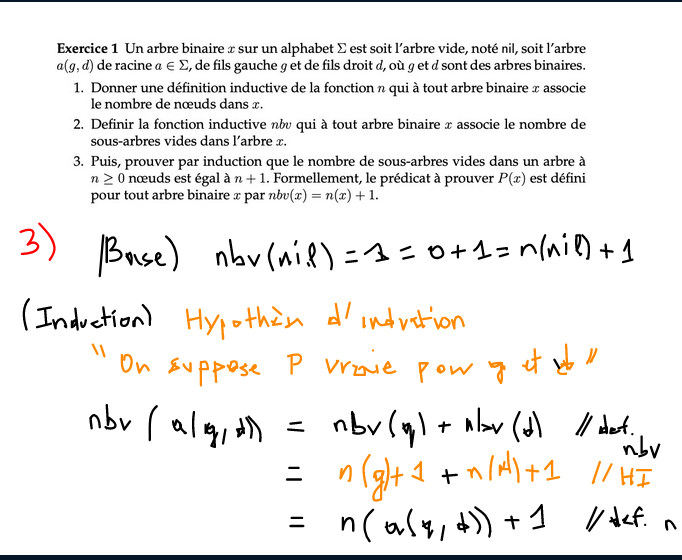
\includegraphics[scale = 0.5]{ex1.3}
      \end{figure}
\end{enumerate}

\section*{Exercice 2}
\underline{Remarque} : $score(K) := n_{1}.n_{2} + score(n_{1} )+ score(n_{2})$ (score avec k boîtes) L'induction est une bonne idée.\\
$P(K) : score(K) = \dfrac{K(K-1)}{2}$, quelque soit la stratégie\\

\underline{cas de base}: K = 1 : $score(1)=0$ et $\dfrac{1(1-1)}{2}=0$ donc P(1) est vrai\\

\underline{cas induction}: On suppose P(k) vrai pour $k<n$. On veut montrer P(n+1):\\
Notre stratégie nous dit de dépiler $n_{1}$ et $n_{2 }$ équivaut à $ n+1$  $(1 \leq n_1 \leq n)$ \\
$score(n+1) = n_{1}(n+1-n_{1}) + score(n_{1}) + score (n+1-n_{1})$ \\
$score(n+1)=n_{1}(n+1-n_{1}) + \dfrac{n_{1}n_{1}-1}{2} + \dfrac{(n+1-n_{1})(n-n_{1})}{2}$
On a montré P(k) vraie pour tout k\\
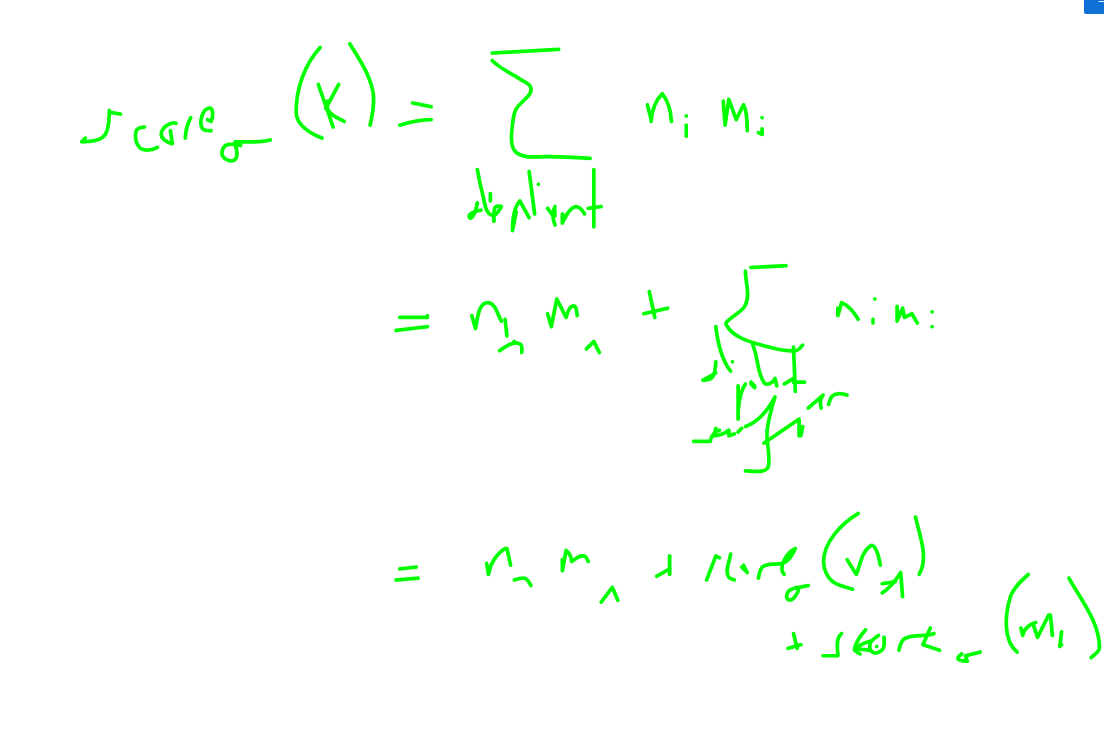
\includegraphics[scale = 0.3]{ex2}

\section*{Exercice 3}
\begin{enumerate}
  \item Longueur 2 : $00,11$\\
    Longueur 3 : $000,010,101,111$\\
  \item $\epsilon ,0,1 \in L$\\
    et si $m \in L$, alors $0m0 \in L$ et $1m1 \in L$\\
    $L_{0} \leq L$:\\

    \underline{cas de base}: $\epsilon , 0,1 \in L $ . \emph{ok}\\

    \underline{cas induction}: Soit $m \in L_0$ \\
    par \emph{H.I.} : $m \in L$
    Donc $0m0 \text{ et } 1m1 \in L $

    l'autre sens, $L \leq L_{0}$ : Induction sur la longueur des palindromes.\\

    \underline{cas de base} : $l = 0$, on a bien $\epsilon \in L_{0}$ . ok\\
    $l=1$, on a bien $0,1\in L_{0}$\\

    \underline{casinduction} : Soit $m \in L$ de taille $l+1$\\
    \emph{ \underline{ H.I. } : si $\omega \in L$, avec $|\omega|\leq l$, alors $\omega \in L_{0}$}\\
    %$ l+1 \req l $ donc $ m = a m' a $ et $ m' \in L $\\
    H.I. : $m' \in L_0$ car $|m'| = |m| - l \leq l$\\
    Par définition de $L_{0} : am'a \in L_{0} $donc $m \in L_{0}$\\
    donc $L = L_{0}$\\

  \item \#palindromes(P) = 1 si P = 0\\
    = 2 si P = 1\\
    ...\\
    =2*\#palindromes(P-2)\\

    \#palindromes(351) = $2^{351/2}$\\
    Donc : \#pal(P)=$2^{P/2}$ si pair et $2^{(P+1)/2}$ si impair.\\
    avec K symboles ; $\# pal_k(P)=k^{P/2}$ si pair ou $\# pal_{k}(P)=k^{(P+1)/2}$\\
\end{enumerate}

\section*{Exercice 4}
 \begin{figure}[!h]
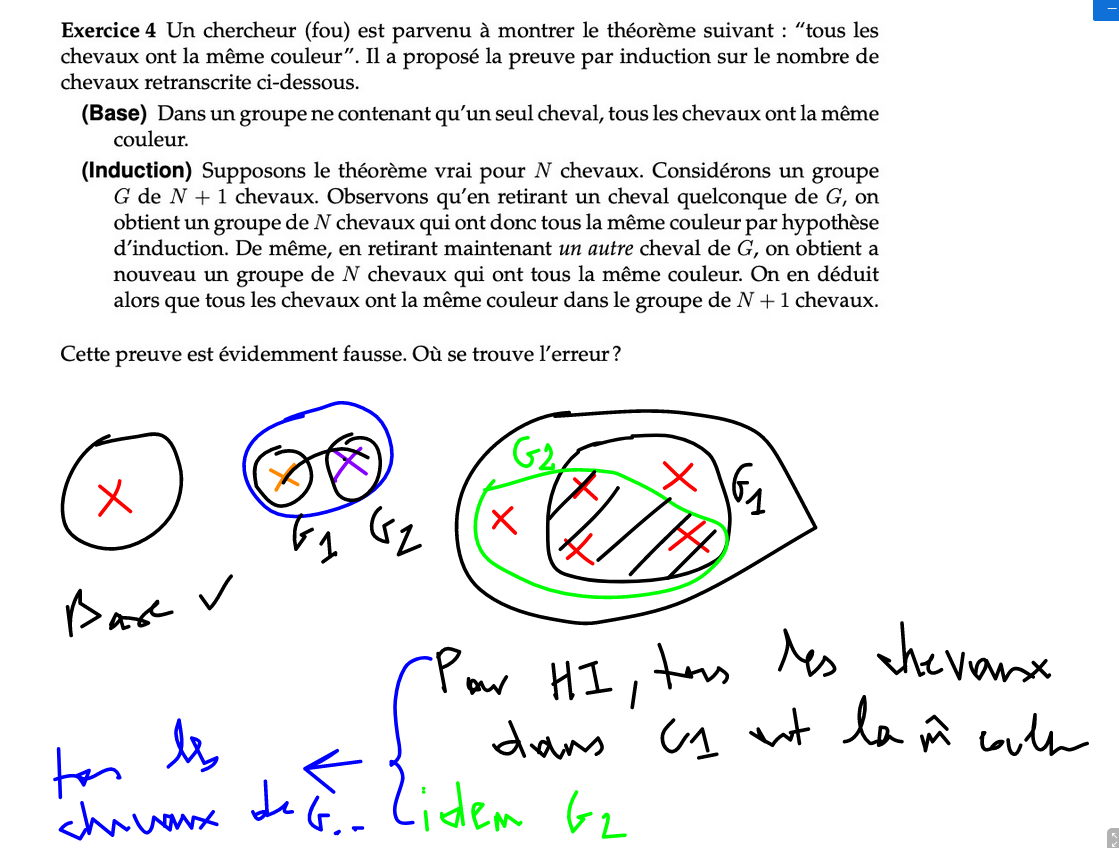
\includegraphics[scale=0.3]{ex4}
c'est l'exercice 4.\\
\end{figure}



\section*{Exercice 8}
 \begin{figure}[!h]
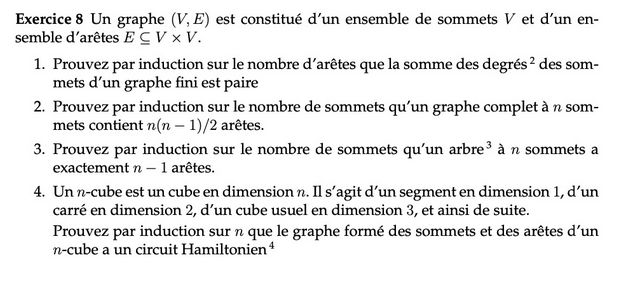
\includegraphics[scale=0.5]{ex8}
\end{figure}
\begin{enumerate}
  \item \underline{cas de base} : $E=\varnothing$.\\
    pour tout noeud n, degrès(n) = 0, c'est pair !\\
    \underline{induction} : On suppose $P_{1}$  vraie pour $G$.\\
    $\sum_{n\in (G + arrete v_{1}-v_{2})}degres(n) = \sum_{n\in G}degres(n) +\underset{V_{1}}{1} +\underset{V_{2}}{1}$, donc c'est toujours pair!\\
  \item \underline{Base} : n = 1 sommet $\longrightarrow$ aucune arète.\\
    $1(1-1)/2=0 $ arète, donc c'est bon.\\
    \underline{Induction} : On suppose $P_{2}$ vraie pour G complet à n sommets.\\
    on obtient $G'$ en ajoutant n arètes à $G$.\\
    $nb_arete(G') = nb_arete(G)+n=\dfrac{n(n-1)}{2}+n$, c'est bon !\\
  \item \underline{Base} : arbre avec 1 sommet $\longrightarrow$ 0 arète, c'est bon !\\
    \underline{Induction} : On suppose $P_{3}$ vraie pour tout arbre ayant $k\leq n$ sommets.\\
    g possède $n_{1}$ sommets, $n_{1}-1$ arètes,\\
    d possède $n_{2}$ sommets, $n_{2}-1$ arètes,\\
    avec $n_{1}+n_{2} = n$\\
    donc $nb\_{aretes(A)}=2+nb\_a(g)+nb\_{a}(d) + 2 = ...$\\
    \item
\end{enumerate}

\end{document}
